\documentclass[a4paper , 12pt]{article}
\usepackage[utf8]{inputenc}
\usepackage{color,soul}
\usepackage[english, francais]{babel}
\usepackage[T1]{fontenc}
\usepackage{graphicx}    % pour inclusion d'image
\usepackage[colorlinks=true]{hyperref}
\usepackage{setspace}
\usepackage{makeidx}
\usepackage{latexsym}
\usepackage{amssymb}
\usepackage{amsmath}
\usepackage{enumitem}
\usepackage{listings}

\usepackage{fancyhdr}
\lhead{Techniques à Objets Avancés}
\rhead{M1 ALMA }
\lfoot{Université de Nantes}
\rfoot{2011-2012 }
\renewcommand{\footrulewidth}{1px}
\pagestyle{fancy}

%% \lstset{
%% basicstyle=\ttfamily\small, %
%% identifierstyle=\color{colIdentifier}, %
%% keywordstyle=\color{colKeys}, %
%% stringstyle=\color{colString}, %
%% commentstyle=\color{colComments}
%% language=java

%% }*/

\title{\bf Eclipse Vision System Plugin}
\author{Diallo Algassimou}

\begin{document}
\maketitle
\tableofcontents

\part*{Présentation générale}
\section{Introduction}
Eclipse Vision System permet de détecter des faits à partir d'un flux d'images et de créer des posts sur un réseau social. L'origine du flux d'images, les traitements apportés aux images ainsi que les faits recherchés dans celles-ci et les posts publiés sur un réseau social sont autant de points de variations qui sont pris en compte par Eclipse Vision System.

\section{Architecture}
Eclipse Vision System definit deux plugins pour des points d'extensions d'eclipse :
\begin{itemize}
\item actionSets (pour lancer le système) systemVideo
\item PreferencePages (Permet d'avoir une page de preferences pour notre système) PreferencePages
\end{itemize}

\begin{figure}
  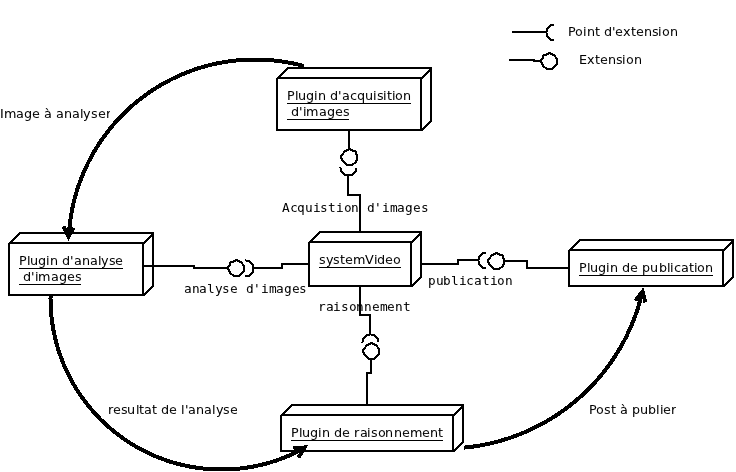
\includegraphics[scale=0.5]{images/architecture.png}
  \caption{Architecture}
  \label{fig:architecture}
\end{figure}

systemVideo est le plugin centrale de notre système. Il fournit quatres points d'extensions qui permettent de capturer toutes les variations possibles dans l'utilisation du système. Ces points d'extensions sont les suivants:
 
\begin{itemize}
\item {\it imageAcquisitionExt} : point d'extension pour les plugins d'acquisition (capture) d'images; 
\item {\it imageAnalysisExt} : point d'extension pour les plugins d'analyse d'images;
\item {\it imageReasonigExt} : point d'extension pour les plugins de traitement d'images ou le raisonnement avant publication; 
\item {\it imagePublicationExt} :point d'extension pour les plugins de publication de posts.
\end{itemize}  
Les plugins suivants ont été dévéloppés et peuvent être utilisés : 
\begin{itemize}
\item {\bf imageAcquisitionCamera} : plugin de capture d'une image à partir d'une webcam; 
\item {\bf imageAcquisitionVideo} :  plugin de capture d'une image à partir d'une video;
\item {\bf imageAnalysis} : plugin d'analyse d'une image (reconnait des visages dans une image); 
\item {\bf imageReasoningSimple} : Publie si l'image contient plus de deux visages ;
\item {\bf imagePublishBlogger} :  publie le message "Nous avons plus de deux visages" sur un google blog.
\end{itemize}  

\part*{Tutorial}
\section{PagePreference}
\begin{figure}
  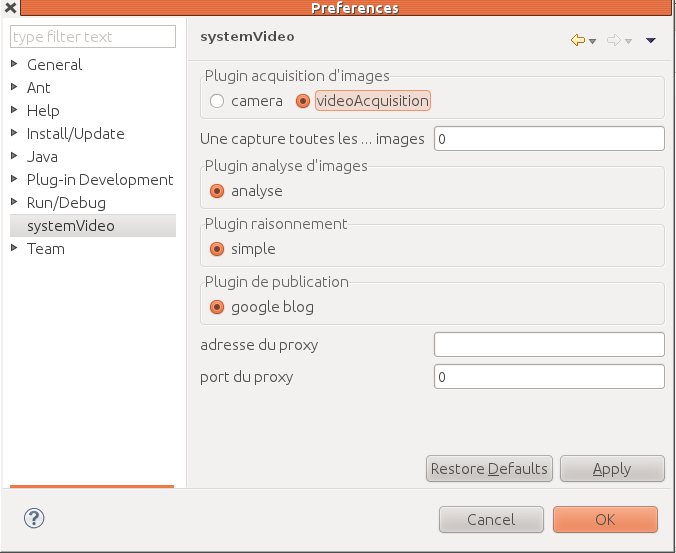
\includegraphics[scale=0.45]{images/preference.png}
  \caption{Page de préferences}
  \label{fig:preferences}
\end{figure}

Pour chacun des points d'extensions l'utilisateur peut choisir le plugin qu'il veut utiliser parmi tous ceux disponibles, et aussi il peut renseigner l'adresse d'un serveur proxy et le port de celui-ci.

\section{exécution}
Dans cette exécution nous allons considérer que les options ont été fixées comme le montre la figure \ref{fig:preferences}.
\subsection{imageAcquisitionVideo}
Ce plugin va capturer les images apartir d'une video pour cela il va demander le chemin de la video (figure \ref{fig:fichier_video}).
\begin{figure}
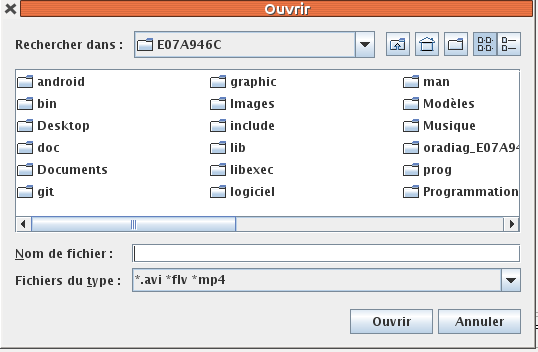
\includegraphics[scale=0.4]{images/fichier_video.png}
\caption{Chemin du fichier video}
\label{fig:fichier_video}
\end{figure}
\subsection{imageAnalysis}
Ce plugin analyse une image à la recherche de visages. Pour cela il a besoin d'un fichier permettant de definir ce qu'est un visage. Ce fichier est fourni par default avec les sources de openCV il suffit de renseigner le chemin du fichier (haarcascade\_frontalface\_alt.xml) dans la fenêtre qui s'ouvre (voir figure \ref{fig:haar}).

\begin{figure}
  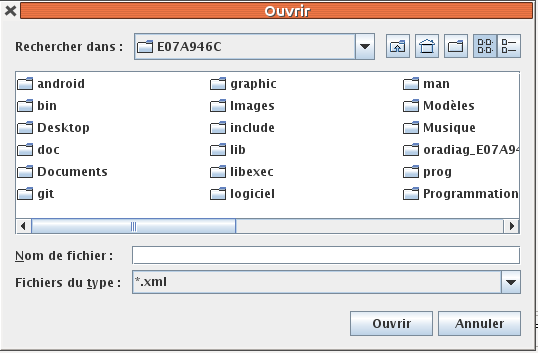
\includegraphics[scale=0.5]{images/figureHaar.png}
  \caption{fichier définissant un visage}
  \label{fig:haar}
\end{figure}

\subsection{imageReasoning}
Ce plugin compte le nombre d'images trouvées par le plugin précedent et post un billet sur le blog si le nombre de visage depasse un certains nombre (Ce nombre est renseigné par l'utilisateur comme le montre la figure \ref{fig:nombre_visages}).

\begin{figure}
  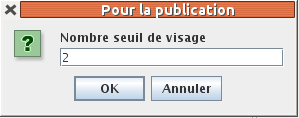
\includegraphics[scale=0.5]{images/nombre_visages.png}
  \caption{Le nombre seuil de visages}
  \label{fig:haar}
\end{figure}

\subsection{imagePublishBlogger}
Ce plugin permet la publication de post sur un blog google. Pour cela il demande en parmatres les identifiants de connexion ainsi le nom de l'auteur du post (voir figure \ref{fig:google}).

\begin{figure}
  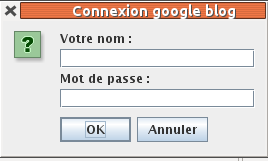
\includegraphics[scale=0.45]{images/google.png}
  \caption{identifiants de connexion compte google}
  \label{fig:google}
\end{figure}

\part*{Utilisation avancée}
Comme le montre la figure \ref{fig:architecture} systemVide définit quatre points d'extensions. Pour ecrire un plugin pour systemVideo on choisit l'un de ces points d'extensions et on definit une classe qui implemente l'interface du point d'extension.

Notre système est un chainage de plugin car le plugin d'acquistion d'image capture une image et la passe au plugin d'analyse qui lui analyse l'image et passe ces résultats au plugin de raisonnement qui traite les résultats et decide ou non de publier.

  \section{Points d'extension et interfaces} 
  \subsection{acquistion d'image}
  L'interface de ce point d'extension est la suivante :
  \lstinputlisting{interfaces/IImageAcquisition.java}
  \subsubsection*{méthod run}
  Cette méthode est appelé par le plugin centrale (systemVideo). elle lance réellement l'exécution du système.
  \subsubsection*{méthod init}
  Cette méthode est appelé pour initialiser le plugin. Elle est appelé avant la methode run et peut être utilisé pour demander des informations à l'utilisateur (chemin d'un fichier , un identifiant etc).

  \subsubsection*{méthod setImageanalysis}
  
  \subsection{analyse d'image}
 \lstinputlisting{interfaces/IImageAnalysis.java}
  \subsection{raisonnement}
 \lstinputlisting{interfaces/IImageReasoning.java}
  \subsection{publication de post}
  \lstinputlisting{interfaces/IImagePublish.java}
  \subsubsection{Architecture globale}
  \begin{enumerate}
  \item {\bf VisonSystem} : VisonSystem est le plugin de central. Ce plugin fournit quatre points d'extensions spécifiques pour tout le processus de traitement et définit les interfaces que devront implémenter les plugins clients; A savoir {\it IImageAcuquisition}, {\it IImageAnalysis}, {\it IImageReasoning}, {\it IImagePublication}.
  \item {\bf imageAcquisitionCamera} : plugin d'acquisition (capture) d'une image à partir d'une video. 
  \item {\bf imageAcquisitionVideo} :  plugin d'acquisition (capture) d'une image à partir d'une webcam. \\
    Ces deux plugins définissent chacun une extension pour le point d'extension prévu à cet effet par visionSystem. La bibliothèque utilisée ici pour la capture est la bibliothèque {\bf xuggler}. Chacun de ces plugins possèdent dans sa classe d'implémentation un objet de type IImageAnalysis qui est ue interface définissant une méthode d'analyse. Le mode d'opération de ces deux plugins est le même : capture une image , instancie un objet de type IImageAnalysis et délègue l'analyse de cette image à l'objet IImageAnalysis.
    ...
  \item {\bf imageAnalysis} : plugin d'analyse d'une image. L'analyse de l'image quand à elle a été faite avec le bibliothèque {\bf OpenCv}. Ce plugin définit lui aussi un obejt de IImageReasoning. Ce plugin récoit l'image à traiter de l'un des deux plugins précédents. L'analyse de l'image est effectué puis l'image est aisni délégué au plugin imageReasonig qui lui se charge du traitement final avant la publication. 
    ...
  \item {\bf imageReasoning} : Ce plugin possède en son sein une liste d'image à publier dans laquelle il range au fur et à mesure les images qui devront être publiées. ...
  \item {\bf imagePublication} : Plugin de publication d'image, recoit les images à publier du plugin imageReasoning puis procède à la publication de celle ci.
    
    Comme on peut le constater les différents plugins présentés s'appuient sur des bibliothèques tierces. De ce fait nous créons des plugins qui regroupent ces bibliothèques qui deviennent ainsi des "repository" de bibliothèques tierces. Ceci est une approche parmi tant d'autre. l'avantage de cette approche est qu'elle évite une duplication des archives des bibliothèques dans tous les plugins utilisant ces bibliothèques. Si un plugin utilise une librairie, il suffira juste d'établir une dépendance avec le plugin (repository) contenant cette librairie. Ceci nous emmène donc à créer les deux plugins suivants : 
  \item {\bf javacvPlugin} : repository de plugin pour javaCv  
  \item {\bf xugglerPlugin} : repository de plugin pour xuggler 

  \end{enumerate}


  \section{Conception}
  Le processus de traitement de l'image suis une séquence bien définie. Le
  \section{}
\end{document}
